% Lorentz.tex      pdflatex ZhCvGo15
% Diffuse globally, compute locally: a cyclist tale
% Tingnan Zhang, Daniel I. Goldman and Predrag Cvitanovi\'c

%\section{Diffusion in periodic arrays}
%\label{s-DiffPerArr}

\begin{figure}[htbp]
  \begin{center}
    (a)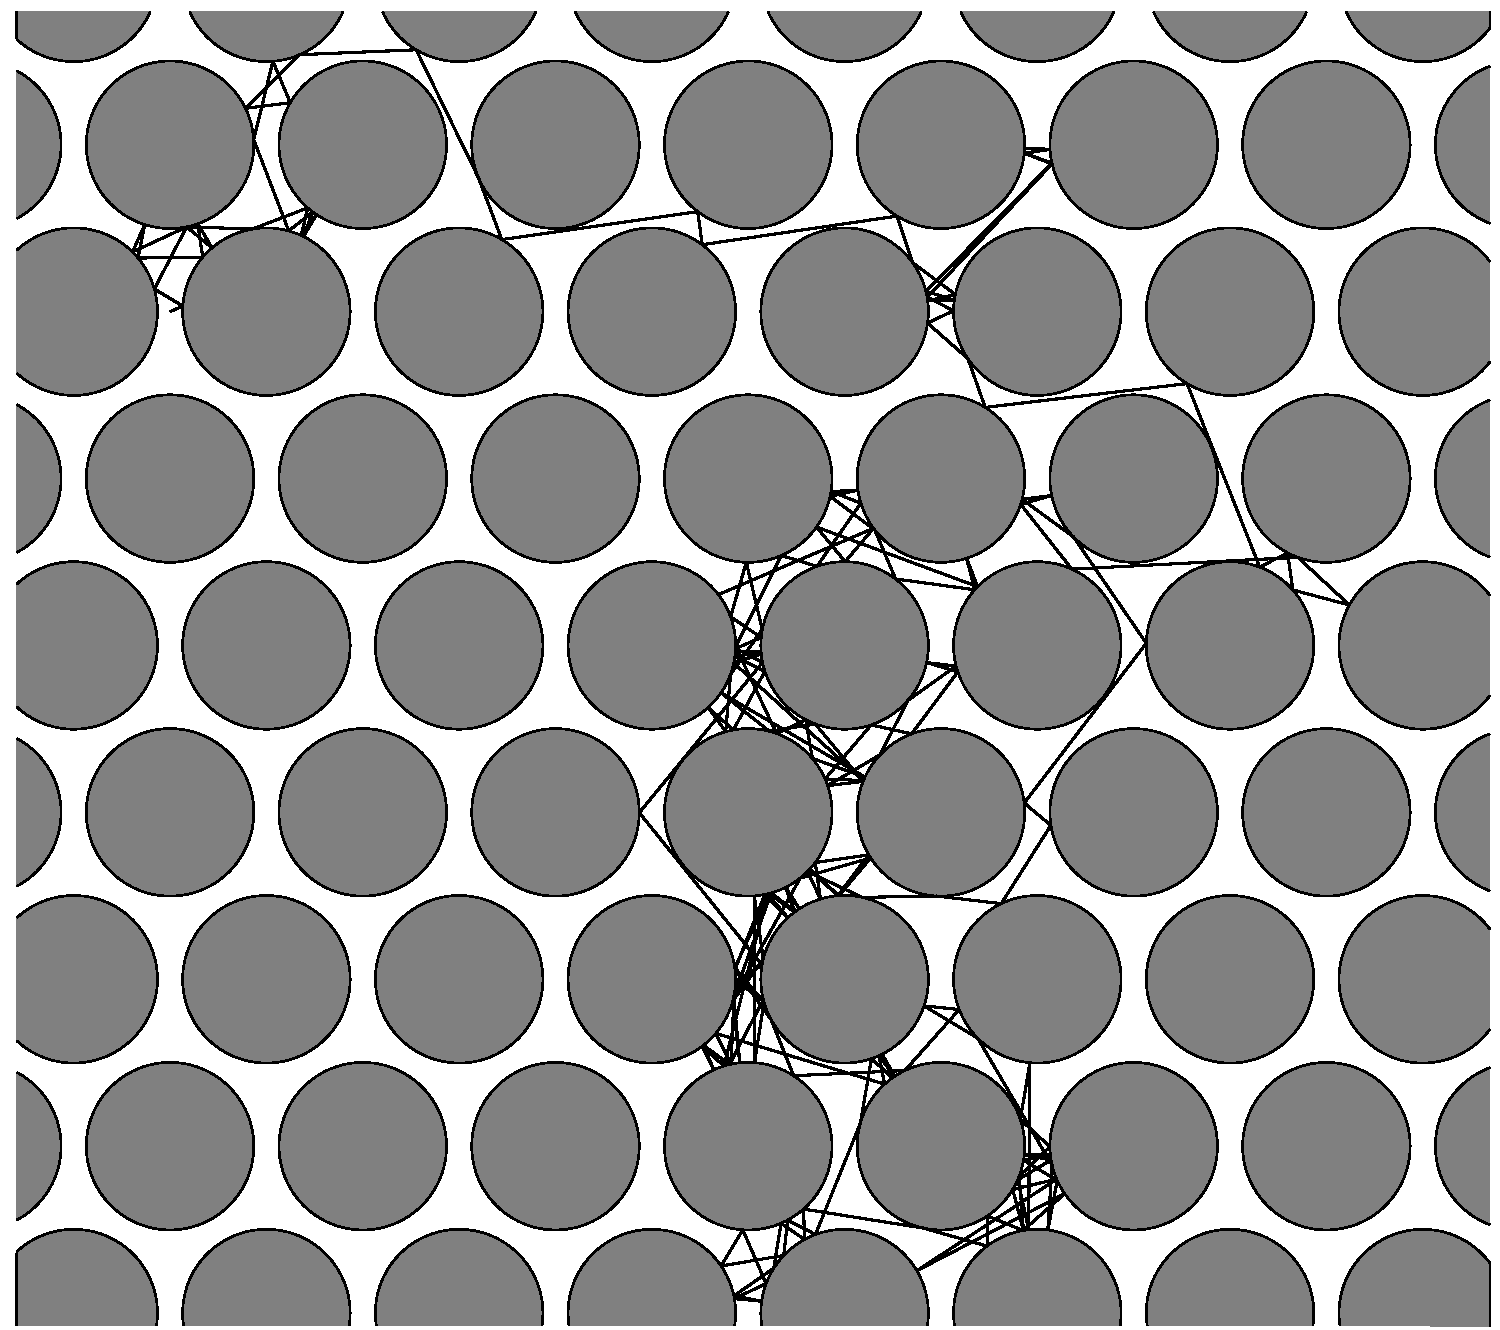
\includegraphics[width=0.45\textwidth]{diffuseChaoticBouncing}
    (b)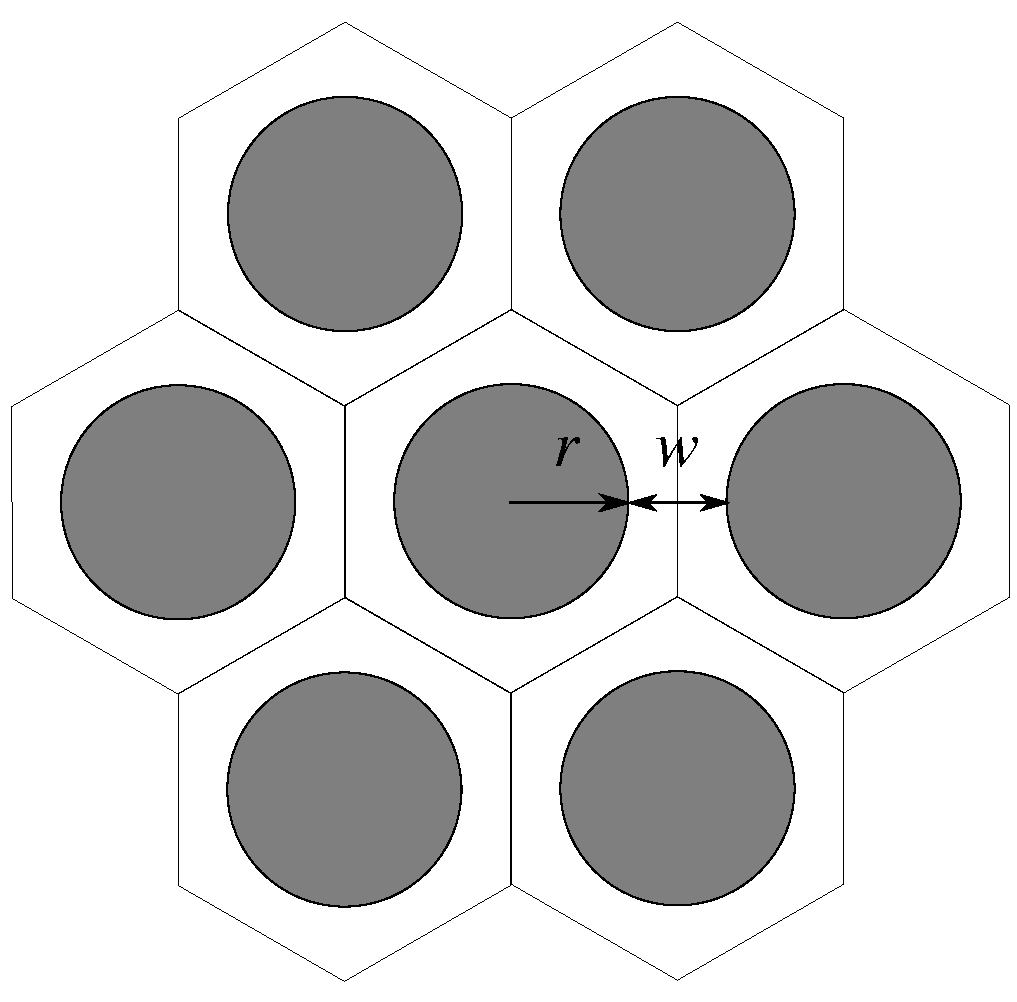
\includegraphics[width=0.45\textwidth]{diffuseLorentzGasParams}
  \end{center}
  \caption[]{\label{fig-chaoticBouncing}
  Motion in the Lorentz gas system. (a)  The chaotic trajectory of a
  ``gas'' particle bouncing in the array of disks  arranged in a
  hexagonal lattice pattern. The distance between disks are close  enough
  such that the particle has no infinite free flight (finite horizon).
  (b) A portion of the triangular Lorentz gas    system. The ratio of
  distance $w$ between the nearest pair of disks to the    disk radius
  $r$ determines the dynamical properties in the system.
  }
\end{figure}

The $2$\dmn\ Lorentz gas is an infinite scatterer array in which
diffusion of a light molecule in a gas of heavy scatterers is modeled by
the motion of a point particle in a plane bouncing off an array of
reflecting disks. The Lorentz gas is called ``gas'' because one can
equivalently think of it as consisting of any number of point-like fast
``light molecules'' interacting only with the stationary ``heavy
molecules'' and not among themselves.  As the scatterer array is built up
from only defocusing concave surfaces, it is a pure hyperbolic system,
and one of the simplest nontrivial dynamical systems that exhibits
deterministic diffusion, \reffig{fig-chaoticBouncing}.

% The original Lorentz gas assumed a random distribution of heavy
% scatterers; in this case a probabilistic description is unavoidable.


===================================== TO REUSE ==========================

    \PC{the text from Cvitanovi\'c, Gaspard and Schreiber\rf{CGS92}}
In the periodic Lorentz gas\rf{Lorentz1905}
a point particle reflects elastically off
a periodic array of reflecting disks in a plane.
The system can
be thought of as an unfolding of the Sinai billiard\rf{Sinai70}.
The standard diffusion constant can be defined if the particle has a bounded
free path between any two successive bounces.
An example is a triangular array with sufficiently small
inter-disk spacing.
Unfortunately, as we shall see,
the same mechanism that guarantees a finite horizon
also leads to rather awkward pruning of periodic orbits.


Machta and Zwanzig\rf{MacZwa83} have given numerical results
for the diffusion constant in Lorentz gases,  as well as
estimates based on a random walk approximation. We shall follow
their notation and fix the radius of the disks to 1,
assume unit particle speed, and
denote the spacing between the disks by $w$ (see fig.~1).
The horizon is finite for $w < 4/\sqrt{3}-2 = 0.3094\dots$.
